% Created by tikzDevice version 0.10.1 on 2016-08-08 10:40:20
% !TEX encoding = UTF-8 Unicode
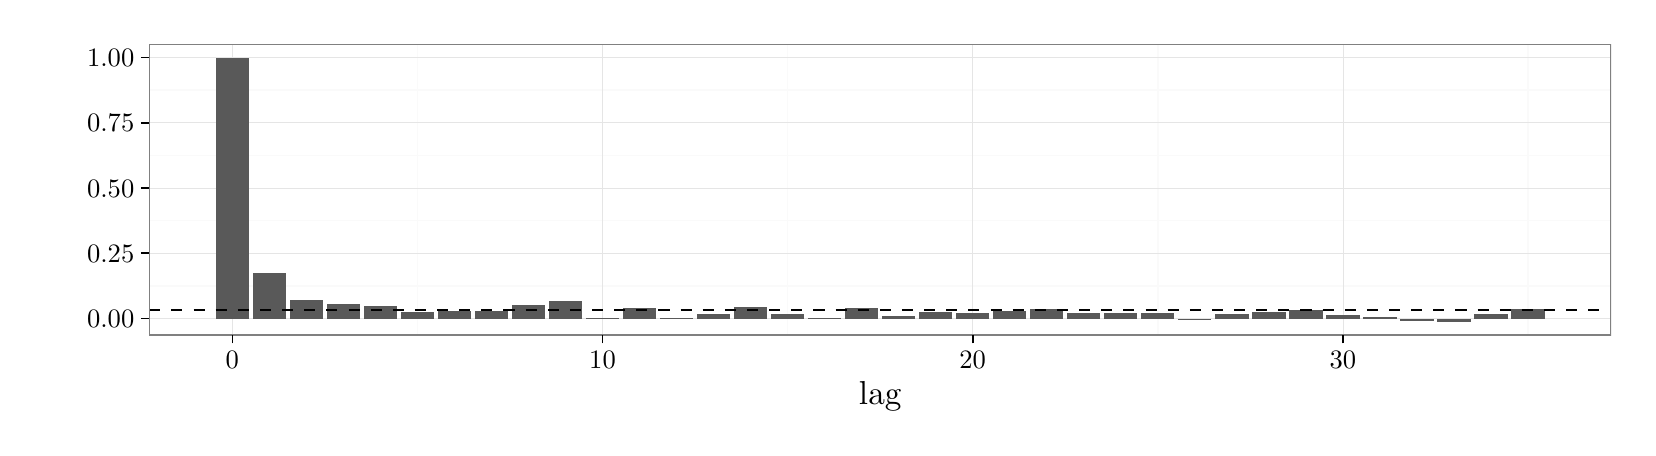
\begin{tikzpicture}[x=1pt,y=1pt]
\definecolor{fillColor}{RGB}{255,255,255}
\path[use as bounding box,fill=fillColor,fill opacity=0.00] (0,0) rectangle (578.16,144.54);
\begin{scope}
\path[clip] (  0.00,  0.00) rectangle (578.16,144.54);
\definecolor{drawColor}{RGB}{255,255,255}
\definecolor{fillColor}{RGB}{255,255,255}

\path[draw=drawColor,line width= 0.6pt,line join=round,line cap=round,fill=fillColor] (  0.00, -0.00) rectangle (578.16,144.54);
\end{scope}
\begin{scope}
\path[clip] ( 43.93, 33.48) rectangle (572.16,138.54);
\definecolor{fillColor}{RGB}{255,255,255}

\path[fill=fillColor] ( 43.93, 33.48) rectangle (572.16,138.54);
\definecolor{drawColor}{gray}{0.98}

\path[draw=drawColor,line width= 0.6pt,line join=round] ( 43.93, 51.22) --
	(572.16, 51.22);

\path[draw=drawColor,line width= 0.6pt,line join=round] ( 43.93, 74.81) --
	(572.16, 74.81);

\path[draw=drawColor,line width= 0.6pt,line join=round] ( 43.93, 98.39) --
	(572.16, 98.39);

\path[draw=drawColor,line width= 0.6pt,line join=round] ( 43.93,121.97) --
	(572.16,121.97);

\path[draw=drawColor,line width= 0.6pt,line join=round] (140.84, 33.48) --
	(140.84,138.54);

\path[draw=drawColor,line width= 0.6pt,line join=round] (274.60, 33.48) --
	(274.60,138.54);

\path[draw=drawColor,line width= 0.6pt,line join=round] (408.37, 33.48) --
	(408.37,138.54);

\path[draw=drawColor,line width= 0.6pt,line join=round] (542.13, 33.48) --
	(542.13,138.54);
\definecolor{drawColor}{gray}{0.90}

\path[draw=drawColor,line width= 0.2pt,line join=round] ( 43.93, 39.43) --
	(572.16, 39.43);

\path[draw=drawColor,line width= 0.2pt,line join=round] ( 43.93, 63.01) --
	(572.16, 63.01);

\path[draw=drawColor,line width= 0.2pt,line join=round] ( 43.93, 86.60) --
	(572.16, 86.60);

\path[draw=drawColor,line width= 0.2pt,line join=round] ( 43.93,110.18) --
	(572.16,110.18);

\path[draw=drawColor,line width= 0.2pt,line join=round] ( 43.93,133.76) --
	(572.16,133.76);

\path[draw=drawColor,line width= 0.2pt,line join=round] ( 73.96, 33.48) --
	( 73.96,138.54);

\path[draw=drawColor,line width= 0.2pt,line join=round] (207.72, 33.48) --
	(207.72,138.54);

\path[draw=drawColor,line width= 0.2pt,line join=round] (341.48, 33.48) --
	(341.48,138.54);

\path[draw=drawColor,line width= 0.2pt,line join=round] (475.25, 33.48) --
	(475.25,138.54);
\definecolor{fillColor}{gray}{0.35}

\path[fill=fillColor] ( 67.94, 39.43) rectangle ( 79.98,133.76);

\path[fill=fillColor] ( 81.31, 39.43) rectangle ( 93.35, 56.05);

\path[fill=fillColor] ( 94.69, 39.43) rectangle (106.73, 46.10);

\path[fill=fillColor] (108.07, 39.43) rectangle (120.11, 44.82);

\path[fill=fillColor] (121.44, 39.43) rectangle (133.48, 44.04);

\path[fill=fillColor] (134.82, 39.43) rectangle (146.86, 41.80);

\path[fill=fillColor] (148.20, 39.43) rectangle (160.23, 42.09);

\path[fill=fillColor] (161.57, 39.43) rectangle (173.61, 42.16);

\path[fill=fillColor] (174.95, 39.43) rectangle (186.99, 44.15);

\path[fill=fillColor] (188.33, 39.43) rectangle (200.36, 45.73);

\path[fill=fillColor] (201.70, 39.43) rectangle (213.74, 39.68);

\path[fill=fillColor] (215.08, 39.43) rectangle (227.12, 43.07);

\path[fill=fillColor] (228.45, 39.43) rectangle (240.49, 39.73);

\path[fill=fillColor] (241.83, 39.43) rectangle (253.87, 41.02);

\path[fill=fillColor] (255.21, 39.43) rectangle (267.25, 43.54);

\path[fill=fillColor] (268.58, 39.43) rectangle (280.62, 41.20);

\path[fill=fillColor] (281.96, 39.43) rectangle (294.00, 39.51);

\path[fill=fillColor] (295.34, 39.43) rectangle (307.37, 43.21);

\path[fill=fillColor] (308.71, 39.43) rectangle (320.75, 40.22);

\path[fill=fillColor] (322.09, 39.43) rectangle (334.13, 41.88);

\path[fill=fillColor] (335.47, 39.43) rectangle (347.50, 41.54);

\path[fill=fillColor] (348.84, 39.43) rectangle (360.88, 42.21);

\path[fill=fillColor] (362.22, 39.43) rectangle (374.26, 42.84);

\path[fill=fillColor] (375.59, 39.43) rectangle (387.63, 41.42);

\path[fill=fillColor] (388.97, 39.43) rectangle (401.01, 41.29);

\path[fill=fillColor] (402.35, 39.43) rectangle (414.39, 41.39);

\path[fill=fillColor] (415.72, 39.32) rectangle (427.76, 39.43);

\path[fill=fillColor] (429.10, 39.43) rectangle (441.14, 40.93);

\path[fill=fillColor] (442.48, 39.43) rectangle (454.51, 41.83);

\path[fill=fillColor] (455.85, 39.43) rectangle (467.89, 42.58);

\path[fill=fillColor] (469.23, 39.43) rectangle (481.27, 40.73);

\path[fill=fillColor] (482.61, 39.43) rectangle (494.64, 39.84);

\path[fill=fillColor] (495.98, 38.62) rectangle (508.02, 39.43);

\path[fill=fillColor] (509.36, 38.25) rectangle (521.40, 39.43);

\path[fill=fillColor] (522.73, 39.43) rectangle (534.77, 41.12);

\path[fill=fillColor] (536.11, 39.43) rectangle (548.15, 42.75);
\definecolor{drawColor}{RGB}{0,0,0}

\path[draw=drawColor,line width= 0.6pt,dash pattern=on 4pt off 4pt ,line join=round] ( 43.93, 42.56) -- (572.16, 42.56);
\definecolor{drawColor}{gray}{0.50}

\path[draw=drawColor,line width= 0.6pt,line join=round,line cap=round] ( 43.93, 33.48) rectangle (572.16,138.54);
\end{scope}
\begin{scope}
\path[clip] (  0.00,  0.00) rectangle (578.16,144.54);
\definecolor{drawColor}{RGB}{0,0,0}

\node[text=drawColor,anchor=base east,inner sep=0pt, outer sep=0pt, scale=  0.96] at ( 38.53, 36.13) {0.00};

\node[text=drawColor,anchor=base east,inner sep=0pt, outer sep=0pt, scale=  0.96] at ( 38.53, 59.71) {0.25};

\node[text=drawColor,anchor=base east,inner sep=0pt, outer sep=0pt, scale=  0.96] at ( 38.53, 83.29) {0.50};

\node[text=drawColor,anchor=base east,inner sep=0pt, outer sep=0pt, scale=  0.96] at ( 38.53,106.88) {0.75};

\node[text=drawColor,anchor=base east,inner sep=0pt, outer sep=0pt, scale=  0.96] at ( 38.53,130.46) {1.00};
\end{scope}
\begin{scope}
\path[clip] (  0.00,  0.00) rectangle (578.16,144.54);
\definecolor{drawColor}{RGB}{0,0,0}

\path[draw=drawColor,line width= 0.6pt,line join=round] ( 40.93, 39.43) --
	( 43.93, 39.43);

\path[draw=drawColor,line width= 0.6pt,line join=round] ( 40.93, 63.01) --
	( 43.93, 63.01);

\path[draw=drawColor,line width= 0.6pt,line join=round] ( 40.93, 86.60) --
	( 43.93, 86.60);

\path[draw=drawColor,line width= 0.6pt,line join=round] ( 40.93,110.18) --
	( 43.93,110.18);

\path[draw=drawColor,line width= 0.6pt,line join=round] ( 40.93,133.76) --
	( 43.93,133.76);
\end{scope}
\begin{scope}
\path[clip] (  0.00,  0.00) rectangle (578.16,144.54);
\definecolor{drawColor}{RGB}{0,0,0}

\path[draw=drawColor,line width= 0.6pt,line join=round] ( 73.96, 30.48) --
	( 73.96, 33.48);

\path[draw=drawColor,line width= 0.6pt,line join=round] (207.72, 30.48) --
	(207.72, 33.48);

\path[draw=drawColor,line width= 0.6pt,line join=round] (341.48, 30.48) --
	(341.48, 33.48);

\path[draw=drawColor,line width= 0.6pt,line join=round] (475.25, 30.48) --
	(475.25, 33.48);
\end{scope}
\begin{scope}
\path[clip] (  0.00,  0.00) rectangle (578.16,144.54);
\definecolor{drawColor}{RGB}{0,0,0}

\node[text=drawColor,anchor=base,inner sep=0pt, outer sep=0pt, scale=  0.96] at ( 73.96, 21.46) {0};

\node[text=drawColor,anchor=base,inner sep=0pt, outer sep=0pt, scale=  0.96] at (207.72, 21.46) {10};

\node[text=drawColor,anchor=base,inner sep=0pt, outer sep=0pt, scale=  0.96] at (341.48, 21.46) {20};

\node[text=drawColor,anchor=base,inner sep=0pt, outer sep=0pt, scale=  0.96] at (475.25, 21.46) {30};
\end{scope}
\begin{scope}
\path[clip] (  0.00,  0.00) rectangle (578.16,144.54);
\definecolor{drawColor}{RGB}{0,0,0}

\node[text=drawColor,anchor=base,inner sep=0pt, outer sep=0pt, scale=  1.20] at (308.04,  8.40) {lag};
\end{scope}
\end{tikzpicture}
